%%
%% This is file `sigconf.tex',
%% generated with the docstrip utility.
\documentclass[sigconf]{acmart}

\AtBeginDocument{%
  \providecommand\BibTeX{{%
    Bib\TeX}}}

\setcopyright{acmlicensed}
\copyrightyear{2018}
\acmYear{2018}
\acmDOI{XXXXXXX.XXXXXXX}

\acmConference[Conference acronym 'XX]{Make sure to enter the correct
  conference title from your rights confirmation email}{June 03--05,
  2018}{Woodstock, NY}
\acmISBN{978-1-4503-XXXX-X/2018/06}

% Text color support
\usepackage{xcolor}

% Dependencies for the framework, algorithm, and measured-result plots migrated from the prior manuscript.
\usepackage{algorithm}
\usepackage{algpseudocode}
\usepackage{tikz}
\usetikzlibrary{arrows.meta,positioning}
\usepackage{pgfplots}
\pgfplotsset{compat=1.18}
\usepgfplotslibrary{groupplots}
\setlength{\emergencystretch}{1em}


\begin{document}
\title{Decision-Model-Guided Function Calling with Cumulative Verification Feedback}

\author{Minhyeong Yu}
% \authornote{Both authors contributed equally to this research.}
\affiliation{%
  \institution{Enhans}
  \city{Seoul}
  \country{South Korea}}
\email{minhyeong@enhans.ai}


\author{Wonduk Seo}
\correspondingauthor
\affiliation{%
  \institution{University College London}
  \city{London}
  \country{United Kingdom}}
\email{wonduk.seo.26@ucl.ac.uk}

% \author{Valerie B\'eranger}
% \affiliation{%
%   \institution{Inria Paris-Rocquencourt}
%   \city{Rocquencourt}
%   \country{France}
% }


\renewcommand{\shortauthors}{Trovato et al.}

\begin{abstract}
\input{sec/abstract}

Reliable function calling requires Large Language Models (LLMs) to choose appropriate functions and generate arguments that match user intent. However, even syntactically valid calls can be semantically wrong, for instance by selecting the wrong function or producing mismatched arguments. Prior work uses verification and iterative refinement, but it remains difficult to efficiently carry verification feedback forward across attempts. In this paper, propose \textbf{Decision-Model-Guided Function Calling (DMFC)}, an inference-time framework that verifies function selection and argument correctness with separate binary judgments and then refines calls using cumulative feedback from previously rejected candidates without executing external tools. \textcolor{red}{On Berkeley Function Calling Leaderboard (BFCL), DMFC improves accuracy from 64.1\% to 74.8\% with GPT-5-nano and from 81.1\% to 82.1\% with GPT-5.4-mini. Retaining verification history further outperforms using only the latest feedback by 1.1 percentage points} highlighting the value of cumulative verification for reliable function calling.
\end{abstract}


\begin{CCSXML}
<ccs2012>
 <concept>
  <concept_id>00000000.0000000.0000000</concept_id>
  <concept_desc>Do Not Use This Code, Generate the Correct Terms for Your Paper</concept_desc>
  <concept_significance>500</concept_significance>
 </concept>
 <concept>
  <concept_id>00000000.00000000.00000000</concept_id>
  <concept_desc>Do Not Use This Code, Generate the Correct Terms for Your Paper</concept_desc>
  <concept_significance>300</concept_significance>
 </concept>
 <concept>
  <concept_id>00000000.00000000.00000000</concept_id>
  <concept_desc>Do Not Use This Code, Generate the Correct Terms for Your Paper</concept_desc>
  <concept_significance>100</concept_significance>
 </concept>
 <concept>
  <concept_id>00000000.00000000.00000000</concept_id>
  <concept_desc>Do Not Use This Code, Generate the Correct Terms for Your Paper</concept_desc>
  <concept_significance>100</concept_significance>
 </concept>
</ccs2012>
\end{CCSXML}

\ccsdesc[500]{Do Not Use This Code~Generate the Correct Terms for Your Paper}
\ccsdesc[300]{Do Not Use This Code~Generate the Correct Terms for Your Paper}
\ccsdesc{Do Not Use This Code~Generate the Correct Terms for Your Paper}
\ccsdesc[100]{Do Not Use This Code~Generate the Correct Terms for Your Paper}

%%
%% Keywords. The author(s) should pick words that accurately describe
%% the work being presented. Separate the keywords with commas.
\keywords{Do, Not, Use, This, Code, Put, the, Correct, Terms, for,
  Your, Paper}
%% A "teaser" image appears between the author and affiliation
%% information and the body of the document, and typically spans the
%% page.
\begin{teaserfigure}
 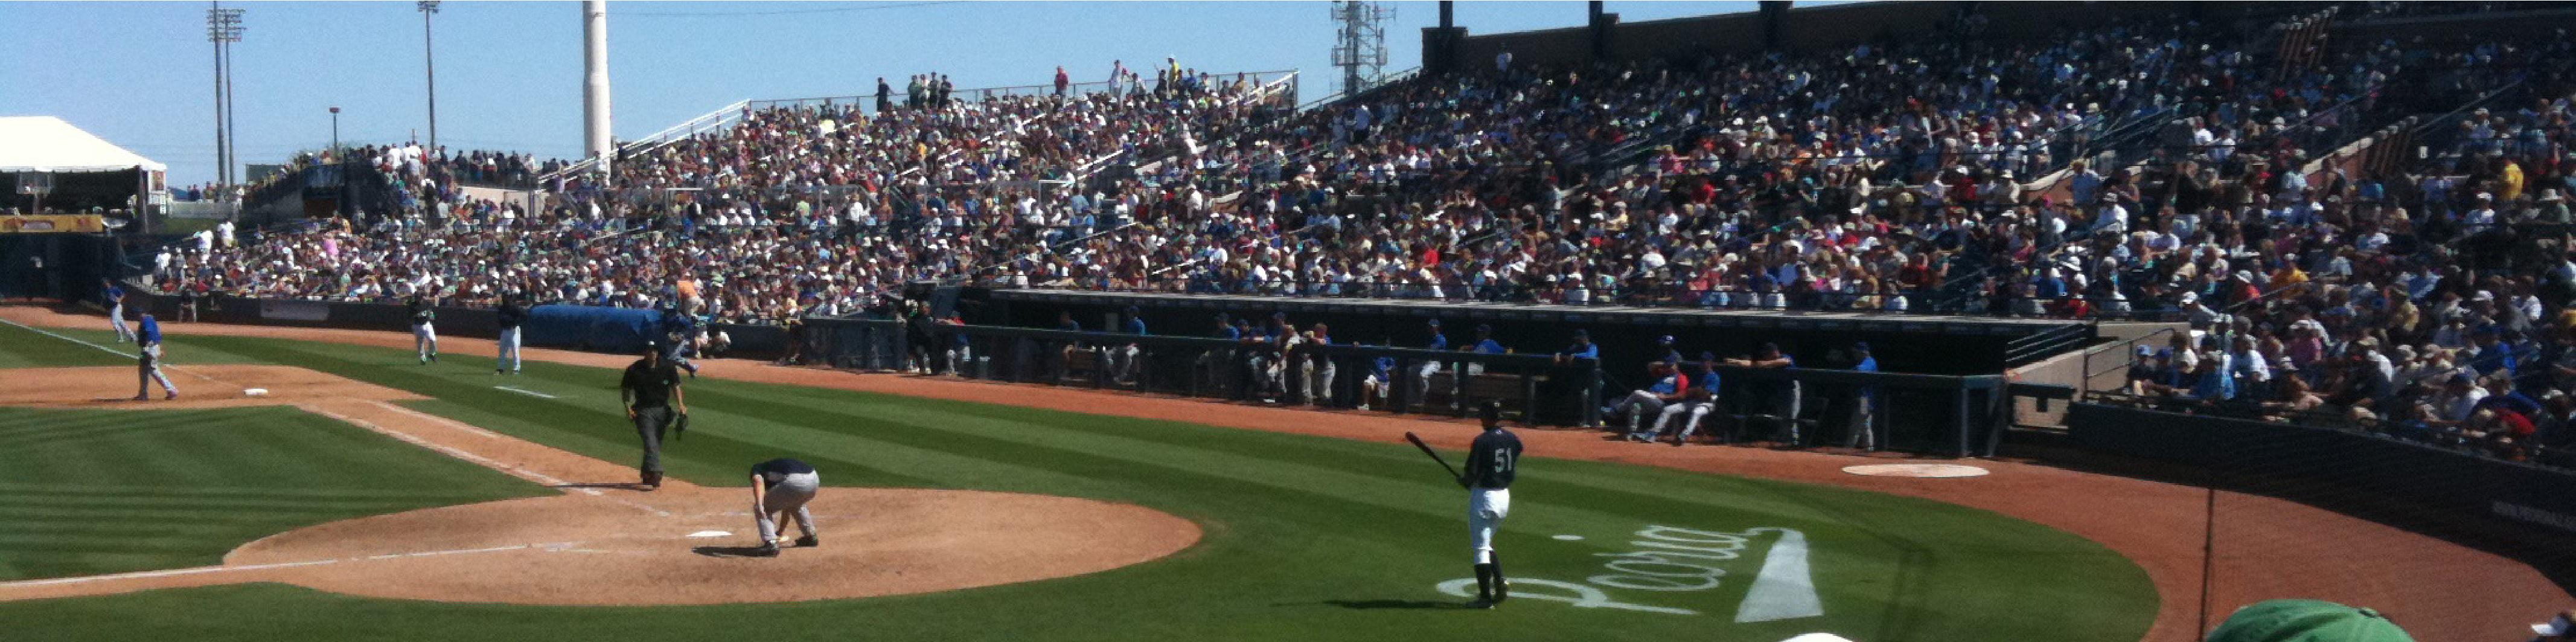
\includegraphics[width=\textwidth]{sampleteaser}
  \caption{Seattle Mariners at Spring Training, 2010.}
  \Description{Enjoying the baseball game from the third-base
  seats. Ichiro Suzuki preparing to bat.}
  \label{fig:teaser}
\end{teaserfigure}

\received{20 February 2007}
\received[revised]{12 March 2009}
\received[accepted]{5 June 2009}

\maketitle



\section{Introduction}
Function calling enables Large Language Models (LLMs) to interact with external tools and APIs by translating natural-language requests into structured function invocations. Given a user request and a set of available functions, an LLM must decide whether to call a function, select the appropriate one, and generate arguments that reflect the user's intent. This capability is central to LLM-based agentic systems that retrieve information, execute actions, and make decisions in external environments. However, syntactic validity does not guarantee semantic correctness: a call can satisfy a schema while selecting the wrong function or filling arguments with incorrect values.

Recent work improves function-calling reliability through schema validation, tool-use verification, and iterative refinement. Schema-based methods enforce structural constraints, while self-refinement uses model-generated critiques to identify and correct errors. Complementary verification-oriented methods explicitly assess function selection and argument values, and feedback-driven agent frameworks revise subsequent actions using signals such as tool-use error detection or execution observations.

Building on these lines of work, recent advances in decision modeling offer a promising approach to providing targeted judgments over candidate outputs. Unlike conventional LLM-based critiques, decision models can produce structured binary judgments to assess whether specific evaluation criteria are satisfied. Recent approaches further explore confidence-aware verification, where lightweight decision models evaluate candidate outputs and selectively defer uncertain cases to stronger judges, improving evaluation efficiency. 

\textcolor{red}{However, turning such judgments into reliable improvements remains challenging. \textbf{First}, structural validation alone cannot determine whether a function call aligns with the user's request, particularly when the correct action is to call no function. \textbf{Second}, function selection and argument generation are distinct error sources: a model may choose the right function but provide wrong arguments, or generate plausible arguments for the wrong function, which calls for fine-grained verification. \textbf{Third}, although iterative refinement can correct mistakes, using only the latest feedback can discard useful signals from earlier failed attempts. These challenges motivate leveraging decision-model verification during refinement while retaining verification history across attempts.
}

To this end, we propose \textbf{Decision-Model-Guided Function Calling (DMFC)}, an inference-time framework that integrates decision-model-based verification with cumulative feedback-driven refinement. \textcolor{red}{DMFC evaluates each generated call with two complementary binary judgments---function selection correctness and argument correctness---in addition to structural schema validation. When a candidate fails verification, the rejected call and its judgments are stored as cumulative feedback and injected into the LLM context to guide subsequent revisions.} A call is accepted only when all applicable verification criteria are satisfied, enabling iterative correction without executing external functions.

\textcolor{red}{We evaluate DMFC using diverse decision-model verifier on the Berkeley Function Calling Leaderboard (BFCL) and xxx.} DMFC improves accuracy from 64.1\% to 74.8\% with GPT-5-nano and from 81.1\% to 82.1\% with GPT-5.4-mini. Retaining verification history further outperforms latest-only feedback by 1.1 percentage points, with the largest gains from preventing unnecessary function calls at the cost of additional inference compute.

Our main contributions are threefold:
\textcolor{red}{
\begin{itemize}
    \item We introduce a decision-model-guided verification framework that explicitly evaluates function selection and argument correctness before execution.
    \item We propose a cumulative feedback-driven refinement mechanism that leverages historical verification judgments to improve subsequent function calls.
    \item We conduct comprehensive experiments and ablation studies to evaluate the effectiveness of the proposed framework in terms of function-calling accuracy, correction behavior, and computational efficiency.
\end{itemize}}

% \section{Problem Definition}
% \input{sec/problem_definition}

\section{Related Work}
\paragraph{Tool use and benchmarks.}
Gorilla studies API-call generation~\cite{patil2024gorilla}; ToolLLM studies tool-use training and evaluation~\cite{qin2024toolllm}. BFCL tests function calling across many settings~\cite{patil2025bfcl}. We use its single-turn Python categories to study decisions made before a function runs. API-Bank offers dialogues with executable API calls~\cite{li2023apibank}. StableToolBench uses caching and simulation to handle changing APIs~\cite{guo2024stabletoolbench}. These suggest broader tests beyond our BFCL subset.

\paragraph{Checks and feedback.}
Self-Refine uses self-generated feedback~\cite{madaan2023selfrefine}, Reflexion uses written feedback~\cite{shinn2023reflexion}, and CRITIC uses feedback from tools~\cite{gou2024critic}. Self-correction can turn correct answers into wrong ones~\cite{huang2024selfcorrect}, so we measure both fixes and new errors. ToolVerifier compares alternatives to check tool choice and parameters separately~\cite{mekala2024toolverifier}. ToolCritic identifies tool-use errors and returns feedback~\cite{hamad2025toolcritic}. \textbf{DMFC} checks complete proposals with a fixed external model through an API and limits repairs.

\paragraph{Accumulated prompts.}
ReAct combines reasoning with actions and observations from an environment~\cite{yao2023react}. Our method uses a similar idea of carrying earlier feedback into the next prompt. Each record contains a proposed function call and verification results, rather than an execution result. The LLM receives all records before the unchanged user request. We do not require a generated reasoning trace or run functions during repair. Many-shot in-context learning often improves as prompts grow to hundreds or thousands of examples, and model-generated rationales kept only when their answers are correct can stand in for human-written ones~\cite{agarwal2024manyshot}. Our records are likewise model-generated examples, labeled by \textit{Jev} instead of reference answers.

\paragraph{\textit{Jev} as a judge.}
Li et al.'s \emph{JEV-as-a-Judge}~\cite{li2026jevjudge} checks finished outputs with probabilities for defined verdicts. If a verdict is uncertain, an independent, stronger judge decides. With fixed rules for when to use the stronger judge, it lowers judging cost while keeping similar accuracy on some tasks. It has limits on difficult reasoning, misleading answer styles, and writing judged without reference information. The study does not test tool or action selection inside agents. \textbf{DMFC} checks proposed function calls and returns failed checks to the same generator for revision. We test the specific design of \textbf{DMFC}.


\section{Methodology}
\begin{figure*}[t]
\centering
\resizebox{\textwidth}{!}{%
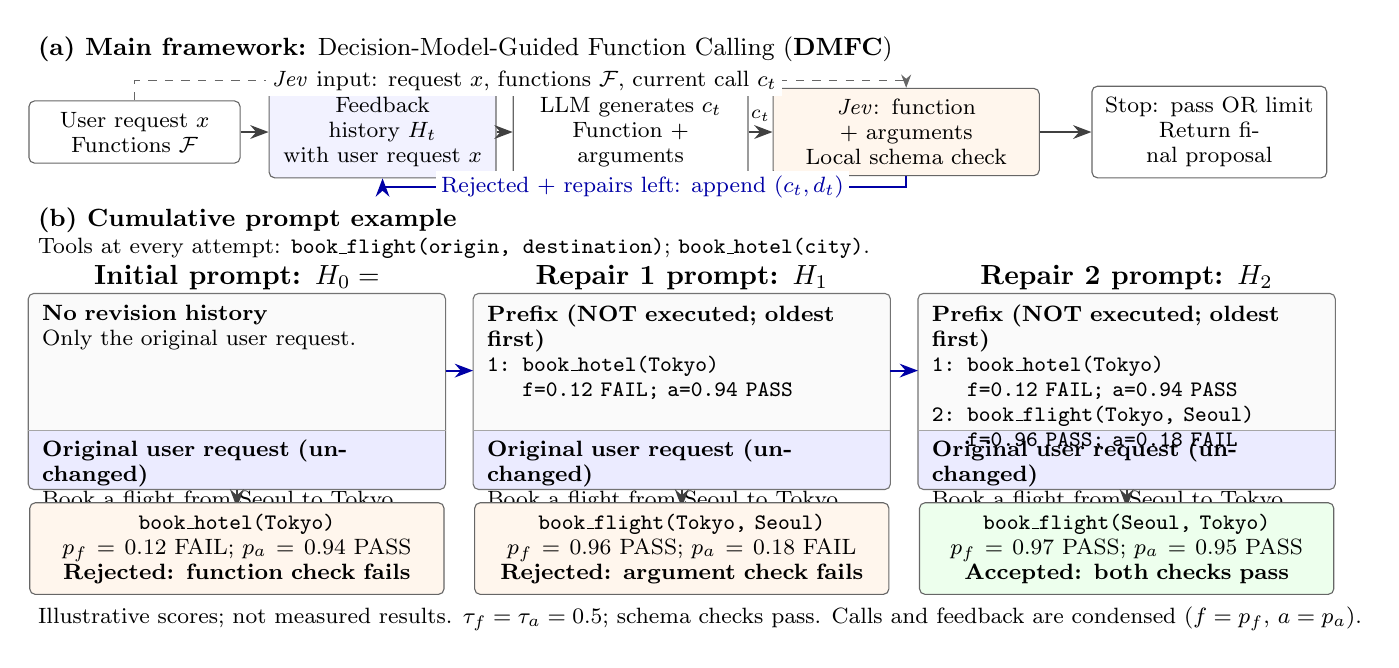
\begin{tikzpicture}[>=Stealth,font=\fontsize{8}{9}\selectfont,
 box/.style={draw=black!60,rounded corners=2pt,align=center,inner sep=4pt,minimum height=0.72cm},
 panel/.style={draw=black!55,rounded corners=2pt},
 flow/.style={->,thick,draw=black!75},
 feedback/.style={->,thick,draw=blue!65!black}]
\node[anchor=west,font=\fontsize{9}{10}\selectfont] at (0,1.05) {\textbf{(a) Main framework:} Decision-Model-Guided Function Calling (\textbf{DMFC})};
\node[box,text width=2.4cm] (request) at (1.35,0) {User request $x$\\Functions $\mathcal{F}$};
\node[box,text width=2.6cm,fill=blue!5] (prompt) at (4.5,0) {Feedback history $H_t$\\with user request $x$};
\node[box,text width=2.7cm] (llm) at (7.65,0) {LLM generates $c_t$\\Function + arguments};
\node[box,text width=3.1cm,fill=orange!7] (judge) at (11.15,0) {\textit{Jev}: function + arguments\\Local schema check};
\node[box,text width=2.7cm] (final) at (15.0,0) {Stop: pass OR limit\\Return final proposal};
\draw[flow] (request)--(prompt);
\draw[flow] (prompt)--(llm);
\draw[flow] (llm)--node[above,font=\fontsize{7}{8}\selectfont] {$c_t$}(judge);
\draw[flow] (judge)--(final);
\draw[->,dashed,draw=black!60] (request.north)--(1.35,0.65)--(11.15,0.65)--(judge.north);
\node[fill=white,inner sep=2pt] at (6.3,0.65) {\textit{Jev} input: request $x$, functions $\mathcal{F}$, current call $c_t$};
\draw[feedback] (judge.south)--(11.15,-0.7)--(4.5,-0.7)--(prompt.south);
\node[fill=white,inner sep=2pt,text=blue!65!black] at (7.8,-0.7) {Rejected + repairs left: append $(c_t,d_t)$};

\node[anchor=west,font=\fontsize{9}{10}\selectfont\bfseries] at (0,-1.12) {(b) Cumulative prompt example};
\node[anchor=west] at (0,-1.48) {Tools at every attempt: \texttt{book\_flight(origin, destination)}; \texttt{book\_hotel(city)}.};
\node[font=\bfseries] at (2.65,-1.85) {Initial prompt: $H_0=\varnothing$};
\node[font=\bfseries] at (8.3,-1.85) {Repair 1 prompt: $H_1$};
\node[font=\bfseries] at (13.95,-1.85) {Repair 2 prompt: $H_2$};

\foreach \x in {0,5.65,11.3} {
  \begin{scope}
    \clip[rounded corners=2pt] (\x,-2.05) rectangle (\x+5.3,-4.54);
    \fill[black!2] (\x,-2.05) rectangle (\x+5.3,-4.54);
    \fill[blue!8] (\x,-3.79) rectangle (\x+5.3,-4.54);
  \end{scope}
  \draw[panel] (\x,-2.05) rectangle (\x+5.3,-4.54);
  \draw[draw=black!35] (\x,-3.79)--(\x+5.3,-3.79);
  \node[anchor=north west,text width=4.95cm,inner sep=0pt] at (\x+0.17,-3.90) {\textbf{Original user request (unchanged)}\\Book a flight from Seoul to Tokyo.};
}
\node[anchor=north west,text width=4.95cm,inner sep=0pt] at (0.17,-2.19) {\textbf{No revision history}\\Only the original user request.};
\node[anchor=north west,text width=4.95cm,inner sep=0pt] at (5.82,-2.19) {\textbf{Prefix (NOT executed; oldest first)}\\
\texttt{1: book\_hotel(Tokyo)}\\
\texttt{\phantom{1: }f=0.12 FAIL; a=0.94 PASS}};
\node[anchor=north west,text width=4.95cm,inner sep=0pt] at (11.47,-2.19) {\textbf{Prefix (NOT executed; oldest first)}\\
\texttt{1: book\_hotel(Tokyo)}\\
\texttt{\phantom{1: }f=0.12 FAIL; a=0.94 PASS}\\
\texttt{2: book\_flight(Tokyo, Seoul)}\\
\texttt{\phantom{2: }f=0.96 PASS; a=0.18 FAIL}};
\foreach \x in {2.65,8.3,13.95} {\draw[flow] (\x,-4.54)--(\x,-4.77);}
\node[box,text width=4.98cm,minimum height=1.05cm,fill=orange!7] at (2.65,-5.29) {\texttt{book\_hotel(Tokyo)}\\$p_f=0.12$ FAIL; $p_a=0.94$ PASS\\\textbf{Rejected: function check fails}};
\node[box,text width=4.98cm,minimum height=1.05cm,fill=orange!7] at (8.3,-5.29) {\texttt{book\_flight(Tokyo, Seoul)}\\$p_f=0.96$ PASS; $p_a=0.18$ FAIL\\\textbf{Rejected: argument check fails}};
\node[box,text width=4.98cm,minimum height=1.05cm,fill=green!7] at (13.95,-5.29) {\texttt{book\_flight(Seoul, Tokyo)}\\$p_f=0.97$ PASS; $p_a=0.95$ PASS\\\textbf{Accepted: both checks pass}};
\draw[feedback] (5.3,-3.03)--(5.65,-3.03);
\draw[feedback] (10.95,-3.03)--(11.3,-3.03);
\node[anchor=west] at (0,-6.18) {Illustrative scores; not measured results. $\tau_f=\tau_a=0.5$; schema checks pass. Calls and feedback are condensed ($f=p_f$, $a=p_a$).};
\end{tikzpicture}}
\caption{\textbf{DMFC} and cumulative prompt feedback. Top: the LLM reads earlier calls and judgments ($H_t$), then the original request ($x$), and generates a call ($c_t$) with a function and arguments. Failed checks add a record for another attempt. Bottom: growing history precedes the unchanged request; new calls appear below. Argument checks concern the proposed function. No function runs during repair.}
\Description{Function-call generation, binary verification, and cumulative feedback over three illustrative attempts.}
\label{fig:loop}
\end{figure*}

\subsection{Task Definition}
Let $x$ be the user request, $\mathcal{F}$ the available functions, and $G$ the generating LLM. A proposal is $c_t=(f_t,a_t)$, with function $f_t$ and arguments $a_t$, or $c_t=\varnothing$ for no call. We study single-call-or-no-call decisions.\footnote{We treat single-turn decisions as the basic unit of function calling. Parallel calling combines multiple such decisions, while multi-turn interactions repeat them with updated context. We therefore evaluate the verification and repair loop on this basic unit and exclude parallel and multi-turn settings from this study.} Local code checks readability, function availability, required arguments, and types. Write $S(c_t)=1$ when these checks pass.

\subsection{Propose and Check a Call}
\paragraph{Binary verification: \textbf{DMFC}.}
For each readable proposal, one \textit{Jev} request checks the function choice and, when a call is present, its arguments:
\begin{align}
 c_t&=G(H_t,x,\mathcal{F}),\\
 p_f^{(t)}&=J_f(x,\mathcal{F},c_t),\qquad
 p_a^{(t)}=J_a(x,\mathcal{F},c_t).
\end{align}
Here $H_t$ contains earlier proposals and feedback and is initially empty. The function \texttt{Noul} question asks whether the function choice, including no call, fits the request. The argument question checks required values, their support in the request, and their parameter roles. For no call, it is skipped and $p_a^{(t)}$ is undefined. A selected function with missing arguments still receives both checks. Both must pass for a call.

\subsection{Accept or Repair a Call}
Acceptance requires the schema check and all required \textit{Jev} checks to pass on the same proposal. The acceptance rule is
\begin{equation}
 A_t=\begin{cases}
 S(c_t)\,\mathbf{1}[p_f^{(t)}\geq\tau_f], & c_t=\varnothing,\\
 S(c_t)\,\mathbf{1}[p_f^{(t)}\geq\tau_f]\,
 \mathbf{1}[p_a^{(t)}\geq\tau_a], & \text{otherwise}.
 \end{cases}
\label{eq:gate}
\end{equation}
\texttt{Noul} returns the probability of yes, with no separate confidence field~\cite{typesafe2026noul,typesafe2026confidence}. We use $\tau_f=\tau_a=0.5$, chosen after runs at 0.8 and 0.7 (Section~\ref{sec:data}).

\begin{algorithm}[t]
\caption{\textbf{DMFC}: verification and prompt repair}
\label{alg:jbfc}
\footnotesize
\begin{algorithmic}[1]
\Require Request $x$, functions $\mathcal{F}$, generator $G$, \textit{Jev} $J$,
\Statex \hspace{\algorithmicindent}repair limit $r$, thresholds $\tau_f,\tau_a$
\State $H\gets[\,]$
\For{$t=0,\ldots,r$}
  \State $c\gets G(\mathrm{Prefix}(H,x),\mathcal{F})$
  \State $(s,e,\mathrm{readable})\gets\mathrm{SchemaCheck}(c,\mathcal{F})$
  \State $p_f,p_a\gets\mathrm{null},\mathrm{null}$
  \If{$\mathrm{readable}$}
    \State $Q\gets\{\mathrm{function}\}$
    \State \textbf{if} $c\ne\varnothing$ \textbf{then} $Q\gets Q\cup\{\mathrm{arguments}\}$
    \State $(p_f,p_a)\gets J(x,\mathcal{F},c,Q)$
  \EndIf
  \State $A\gets\mathrm{Accept}(s,c,p_f,p_a,\tau_f,\tau_a)$ \Comment{Eq.~\ref{eq:gate}}
  \State $d\gets\mathrm{Feedback}(e,p_f,p_a,\tau_f,\tau_a,c)$
  \State \textbf{if} $A=1$ \textbf{or} $t=r$ \textbf{then break}
  \State $H\gets H\mathbin{\Vert}[(c,d)]$
\EndFor
\State \Return $c$ \textbf{if} $A=1$ \textbf{else} $c_0$ \Comment{$c_0$: first proposal}
\end{algorithmic}
\end{algorithm}

\paragraph{Feedback before the user request.}
$H_t$ stores earlier records. The current record $(c_t,d_t)$ pairs proposal $c_t$ with feedback $d_t$ (probabilities, pass/fail flags, thresholds, and local errors). No-call skips the argument check. After rejection, if repairs remain, $\Vert$ adds $[(c_t,d_t)]$, a list containing this one record, to the end of $H_t$:
\begin{equation}
 H_{t+1}=H_t\mathbin{\Vert}[(c_t,d_t)].
\end{equation}
The LLM reads this history before the unchanged request and can change both function and arguments. Schemas remain available; system instructions stay separate.

Algorithm~\ref{alg:jbfc} rechecks up to $r+1$ proposals: the first plus repairs ($r=3$ by default and in experiments). Its \texttt{Prefix} function places JSON records, oldest first, before unchanged original messages. Empty history adds no prefix. Records include round numbers and mark proposals as not executed. Here $s=S(c)$ and $e$ lists local errors. Readable proposals receive \textit{Jev} checks even if their schema fails; unreadable ones receive local feedback. \textit{Jev} never receives history. Unasked $p_a$ stays null. Null required probabilities cannot pass the gate; invalid API responses stop the run. Reference answers stay out of model requests. API errors stop the run after transport retries, separate from repairs.

\subsection{Final Proposal}
When a proposal passes all applicable checks, we return it. If the repair limit is reached first, we return the first proposal, so a repair replaces the generator's answer only once it passes (Table~\ref{tab:rules} compares returning the last). We score the final proposal against the benchmark answers without running the function.


\section{Experiment Setting \& Results}
\subsection{Data and Evaluation}
\label{sec:data}
We prepare 3,051 BFCL examples from seven categories at repository revision \texttt{6ea57973c7a6}\footnote{Full revision: \nolinkurl{6ea57973c7a6097fd7c5915698c54c17c5b1b6c8}. The saved setup lists source URLs, hashes, and format changes.}. Each run uses all examples once. Settings were chosen on these examples (no held-out split): $r=3$ on the first run at threshold 0.8, returning the last proposal; then threshold 0.5 (of 0.7 and 0.5) and the first proposal, after \textbf{DMFC} lowered \nolinkurl{gpt-5.4-mini}'s accuracy.

% BEGIN AUTO CATEGORIES
\begin{table}[t]
\centering\footnotesize
\setlength{\tabcolsep}{4pt}
\begin{tabular}{lrrrrr}
\toprule
 & & \multicolumn{2}{c}{\texttt{gpt-5-nano}} & \multicolumn{2}{c}{\nolinkurl{gpt-5.4-mini}}\\
\cmidrule(lr){3-4}\cmidrule(lr){5-6}
Category & Examples & Direct & \textbf{DMFC} & Direct & \textbf{DMFC}\\
\midrule
Simple Python & 400 & 90.8 & 91.3 & 90.5 & \textbf{91.8}\\
Multiple & 200 & 91.0 & 91.5 & 93.3 & \textbf{95.0}\\
Irrelevance & 240 & 27.2 & 78.2 & 87.1 & \textbf{87.9}\\
Live simple & 258 & 74.3 & 77.8 & 77.1 & \textbf{79.8}\\
Live multiple & 1053 & 67.6 & 71.4 & 75.2 & \textbf{77.4}\\
Live irrelevance & 884 & 48.8 & 65.7 & \textbf{80.7} & 79.4\\
Live relevance$^\dagger$ & 16 & 89.6 & \textbf{91.7} & 79.2 & 83.3\\
\midrule
Total & 3051 & 64.1{\scriptsize$\pm$0.3} & 74.8{\scriptsize$\pm$0.3} & 81.1{\scriptsize$\pm$0.2} & \textbf{82.1}{\scriptsize$\pm$0.1}\\
USD/1k & & 0.056 & 0.210 & 0.703 & 1.137\\
\bottomrule
\end{tabular}
\caption{Accuracy (\%) on all BFCL examples, mean of three runs, $r=3$. Bold: highest per row. Total: mean $\pm$ s.d. over runs. USD/1k: cost per 1,000 requests. $^\dagger$Call presence only; not in the total.}
\label{tab:categories}
\end{table}
% END AUTO CATEGORIES

The original Python abstract syntax tree (AST) checker compares function names and arguments with allowed answers, not execution success; irrelevance categories require no call. Live relevance checks only call presence, so the main score, a micro-average, covers 3,035 examples. BFCL's ``multiple'' categories offer several functions but no parallel calls; we exclude parallel, multi-turn, web-search, memory, and execution categories.

\subsection{Models and Methods}
The generator is the Azure OpenAI deployment \texttt{gpt-5-nano} (\nolinkurl{gpt-5-nano-2025-08-07}), with reasoning effort \texttt{none} and at most 4,096 output tokens; \textit{Jev} is pinned to \texttt{jev-1.13.0}. We use Chat Completions through an APIM gateway and System One directly, and convert BFCL schemas to JSON Schema with API-safe function names. Generations cut off at the output limit or blocked by the provider's filter count as wrong. Direct and \textbf{DMFC} also run on the larger, costlier deployment \nolinkurl{gpt-5.4-mini} (snapshot 2026-03-17) with the same settings. Table~\ref{tab:categories} averages three runs per generator, each with new initial proposals.

We compare seven methods, sharing one initial proposal per example. \emph{Direct} uses the initial proposal; \emph{Schema-only} repairs schema errors. \emph{Self-refine} uses generic self-review in all $r$ repairs, not the full Self-Refine method~\cite{madaan2023selfrefine}. \textbf{DMFC-F} and \textbf{DMFC-A} obtain applicable \texttt{Noul} judgments but expose and require only the function or argument verdict, plus schema checks. \textbf{DMFC-A} accepts no call on schema checks alone. \textbf{DMFC-L} shares \textbf{DMFC}'s settings and initial proposal but shows only the latest rejected proposal and feedback. Neither model sees $r$ and nothing runs before the end, so a larger limit only continues trajectories: the first run ran all methods with $r=2$ and continued them to $r=3$; the \textit{Jev} methods ran again at threshold 0.5 (stated in their feedback) from the same initial proposals, \textbf{DMFC} to $r=10$ for Figure~\ref{fig:repairs}. Like \textbf{DMFC}, methods that stop at a passing proposal return the first if none passes.

% BEGIN AUTO RESULTS
\begin{table}[t]
\centering\small
\setlength{\tabcolsep}{2.7pt}
\begin{tabular}{lrrrrr}
\toprule
Method & Call & Func. & Args. & Sec. & USD/1k \\
\midrule
Direct & 63.8 & 74.8 & 81.2 & 1.30 & 0.056 \\
Schema repair & 65.8 & 76.4 & 81.8 & 1.36 & 0.059 \\
Self-refine & 70.0 & 80.3 & 82.2 & 5.47 & 0.265 \\
\textbf{DMFC-F} & 73.2 & 84.5 & 81.4 & 2.24 & 0.172 \\
\textbf{DMFC-A} & 72.5 & 82.6 & \textbf{82.7} & 2.21 & 0.169 \\
\textbf{DMFC-L} & 73.5 & 84.3 & 82.2 & 2.60 & 0.203 \\
\textbf{DMFC} & \textbf{74.6} & \textbf{85.3} & 82.1 & 2.61 & 0.211 \\
\bottomrule
\end{tabular}
\caption{Methods on all BFCL examples (one run, $r=3$, \texttt{gpt-5-nano}). Bold: highest accuracy per column. Call and function accuracy (\%) exclude live relevance; argument accuracy (\%) uses calls with the correct function.}
\label{tab:main}
\end{table}
% END AUTO RESULTS


% BEGIN AUTO REPAIRS
\begin{figure}[t]
\centering
\definecolor{repaircall}{HTML}{2A78D6}
\definecolor{repairfunction}{HTML}{EB6834}
\definecolor{repaircost}{HTML}{52514E}
\begin{tikzpicture}
\begin{axis}[scale only axis, width=0.80\columnwidth, height=2.0cm, xmin=0.3, xmax=10.7,
  xtick={1,2,3,5,7,10}, xticklabels={{1\\\color{repaircost}0.15},{2\\\color{repaircost}0.18},{3\\\color{repaircost}0.21},{5\\\color{repaircost}0.27},{7\\\color{repaircost}0.32},{10\\\color{repaircost}0.40}}, xticklabel style={align=center},
  ymin=70, ymax=91, ytick={70,75,80,85,90}, ylabel={Accuracy (\%)}, xlabel={Repair limit $r$ (gray: USD per 1,000 requests)},
  axis x line*=bottom, axis y line*=left, ymajorgrids, grid style={black!12},
  tick label style={font=\scriptsize}, label style={font=\scriptsize}, tick align=outside,
  major tick length=2pt, ylabel style={yshift=-3pt},
  legend style={font=\scriptsize, draw=none, fill=none, at={(0.99,0.03)}, anchor=south east,
  legend columns=2, /tikz/every even column/.append style={column sep=6pt}}]
\addplot[color=repaircall, mark=*, mark size=1.5pt, thick] coordinates {(1,72.0264) (2,73.4102) (3,74.5634) (5,75.8484) (7,76.3756) (10,76.7381)};
\addlegendentry{Call}
\addplot[color=repairfunction, mark=square*, mark size=1.5pt, thick] coordinates {(1,82.8007) (2,84.1516) (3,85.3048) (5,86.5898) (7,87.0840) (10,87.4135)};
\addlegendentry{Function}
\node[font=\tiny, anchor=south, yshift=1.5pt, inner sep=1pt] at (axis cs:1,72.0264) {72.0};
\node[font=\tiny, anchor=south, yshift=1.5pt, inner sep=1pt] at (axis cs:2,73.4102) {73.4};
\node[font=\tiny, anchor=south, yshift=1.5pt, inner sep=1pt] at (axis cs:3,74.5634) {74.6};
\node[font=\tiny, anchor=south, yshift=1.5pt, inner sep=1pt] at (axis cs:5,75.8484) {75.8};
\node[font=\tiny, anchor=south, yshift=1.5pt, inner sep=1pt] at (axis cs:7,76.3756) {76.4};
\node[font=\tiny, anchor=south, yshift=1.5pt, inner sep=1pt] at (axis cs:10,76.7381) {76.7};
\node[font=\tiny, anchor=south, yshift=1.5pt, inner sep=1pt] at (axis cs:1,82.8007) {82.8};
\node[font=\tiny, anchor=south, yshift=1.5pt, inner sep=1pt] at (axis cs:2,84.1516) {84.2};
\node[font=\tiny, anchor=south, yshift=1.5pt, inner sep=1pt] at (axis cs:3,85.3048) {85.3};
\node[font=\tiny, anchor=south, yshift=1.5pt, inner sep=1pt] at (axis cs:5,86.5898) {86.6};
\node[font=\tiny, anchor=south, yshift=1.5pt, inner sep=1pt] at (axis cs:7,87.0840) {87.1};
\node[font=\tiny, anchor=south, yshift=1.5pt, inner sep=1pt] at (axis cs:10,87.4135) {87.4};
\end{axis}
\end{tikzpicture}
\caption{\textbf{DMFC} accuracy (\%) by repair limit $r$: one run continued to $r=10$ and cut at each limit ($r=3$ is Table~\ref{tab:main}).}
\label{fig:repairs}
\end{figure}
% END AUTO REPAIRS

\subsection{Measures, Cost, and Uncertainty}
We report call, function, and argument accuracy (the last given the correct function), fixes and new errors, acceptance, and repairs. We compare repairs with Direct, \textbf{DMFC} with \textbf{DMFC-L}, and the two final-proposal rules on matching examples and initial proposals, bootstrapping example IDs 2,000 times (seed 1729) for 95\% intervals after averaging each example over runs.

Costs count all generation and verification work, including the growing history and the shared initial call; times are mean API seconds without retry waits. Prices in USD per million uncached/\allowbreak cached/\allowbreak output tokens are 0.05/\allowbreak 0.005/\allowbreak 0.40 for \texttt{gpt-5-nano} and 0.75/\allowbreak 0.075/\allowbreak 4.50 for \nolinkurl{gpt-5.4-mini}; \textit{Jev} input costs \$0.042 (output free), without gateway fees; one filtered generation without usage is left out.

\subsection{Results}
In Table~\ref{tab:categories}, \textbf{DMFC} raises mean accuracy from 64.1\% to 74.8\% (paired difference 10.7 points, 95\% interval 9.7--11.6; per run 10.8, 10.7, 10.4). Per run, it fixes 323--337 wrong initial proposals, breaks 7--10, and averages 0.64--0.65 repairs; 84--85\% of examples pass, 84--85\% of them correctly. Other numbers are from the first run unless stated.

% BEGIN AUTO RULES
\begin{table}[t]
\centering\footnotesize
\setlength{\tabcolsep}{4pt}
\begin{tabular}{lrrrr}
\toprule
Generator & Direct & Last & First & First $-$ last\\
\midrule
\texttt{gpt-5-nano} & 64.1 & \textbf{75.1} & 74.8 & $-$0.35 [$-$0.68, $-$0.03]\\
\nolinkurl{gpt-5.4-mini} & 81.1 & 80.7 & \textbf{82.1} & +1.37 [0.93, 1.82]\\
\bottomrule
\end{tabular}
\caption{Call accuracy (\%), mean of three runs, when \textbf{DMFC} returns the last or the first proposal if none passes. First $-$ last: paired difference [95\% interval].}
\label{tab:rules}
\end{table}
% END AUTO RULES

\paragraph{Returning the first proposal.}
The rules differ only when no proposal passes; returning the last then makes unverified changes, which per run fix 26--33 calls and break 16--22 with \texttt{gpt-5-nano} but fix 10--14 and break 53--55, mostly correct no-calls, with \nolinkurl{gpt-5.4-mini}. Keeping only accepted changes gains 1.4 points for \nolinkurl{gpt-5.4-mini} and costs \texttt{gpt-5-nano} 0.4 (Table~\ref{tab:rules}).

\paragraph{A larger generator.}
Without \textit{Jev}, \nolinkurl{gpt-5.4-mini} reaches 81.1\%, 6.4 points above \textbf{DMFC} with \texttt{gpt-5-nano} (95\% interval 5.1--7.7), at 3.3 times the cost and under half the time. \textbf{DMFC} raises it in every run, by 1.0 point on average (95\% interval 0.5--1.5); per run, it fixes 55--66 calls and breaks 27--39, mostly no-calls turned into accepted calls.

\paragraph{Comparison of methods.}
In Table~\ref{tab:main}, every repair method beats Direct (paired 95\% intervals above zero): schema repair by 2.0 points, self-refine 6.3, \textbf{DMFC-F} 9.5, \textbf{DMFC-A} 8.7, and \textbf{DMFC-L} 9.8. Self-refine makes four proposals per request yet trails the \textit{Jev}-based methods (1.4 to 1.6).

\paragraph{Why no-call cases gain most.}
Direct calls the one, unrelated function in 179 of 240 Irrelevance examples. \textit{Jev} separates these from the 61 correct no-calls (median function probability 0.09 vs.\ 0.95), and the generator withholds 126 of 156 rejected calls; in live irrelevance, separation is weaker (0.53 vs.\ 0.87), and 160 of 379 are withheld. Where reference calls exist, \textbf{DMFC} rejects 216 of 463 wrong initial calls but fixes only 51: a verdict flags a wrong call, not the right one.

\paragraph{More repairs.}
In Figure~\ref{fig:repairs}, $r=10$ reaches 76.7\%, at 1.6 times the time and 1.9 times the cost of $r=3$; later passing proposals fix 70 examples (59 by withholding a call) and break 4.

\paragraph{Records as in-context examples.}
Each record pairs a call with \textit{Jev}'s verdict, so the history acts as labeled in-context examples, made without reference answers in 0.19~s per label at about \$0.06 per 1,000. As in many-shot learning~\cite{agarwal2024manyshot}, more examples help: with the same attempts, the full history beats the latest record by 1.1 points (\textbf{DMFC} minus \textbf{DMFC-L}, 95\% interval 0.4--1.7), though all are failed attempts at one request.

\subsection{Study Limits}
The verifier can accept a wrong call or share the generator's mistake, and feedback can introduce or reinforce errors. We use two generators, one verifier, and mostly English single-turn requests; Table~\ref{tab:main} and Figure~\ref{fig:repairs} come from one run, and public examples may appear in training data. Ten documented annotation errors stay. Settings were chosen on these examples, so gains may be optimistic; effort \texttt{none} is untuned, and one common limit may favor some methods.


\section{Conclusion}
DMFC combines function and argument judgments with cumulative rejected-call feedback before execution. It improves accuracy for both evaluated generators, with a larger gain for \texttt{gpt-5-nano}. More repairs improve accuracy but increase API time and cost. Comparisons across decision-model families and held-out tuning remain necessary.


\begin{acks}
This work was created as part of the No-More-Slops group activities at Pseudo Lab.

\end{acks}

\clearpage
\bibliographystyle{ACM-Reference-Format}
\bibliography{references}

\end{document}
